% This work is licensed under the Creative Commons
% Attribution-NonCommercial-ShareAlike 4.0 International License. To view a copy
% of this license, visit http://creativecommons.org/licenses/by-nc-sa/4.0/ or
% send a letter to Creative Commons, PO Box 1866, Mountain View, CA 94042, USA.

% (c) Eric Kunze, 2019

%%%%%%%%%%%%%%%%%%%%%%%%%%%%%%%%%%%%%%%%%%%%%%%%%%%%%%%%%%%%%%%%%%%%%%%%%%%%
% Template for lecture notes and exercises at TU Dresden.
%%%%%%%%%%%%%%%%%%%%%%%%%%%%%%%%%%%%%%%%%%%%%%%%%%%%%%%%%%%%%%%%%%%%%%%%%%%%

\documentclass[ %
    ngerman, %
    a4paper, %
    sectionreset, %
    chapterstyle=framed, %
    sectionstyle=pure, %
    titlefont=osfamily %
]{../../texmf/tex/latex/mathscriptMathTUD/mathscriptMathTUD}

\usepackage[order=firstname, fractionappearence=lowerraise]{../../texmf/tex/latex/mathworkMathTUD/mathworkMathTUD}
%\usepackage[presentExercise]{../../texmf/tex/latex/exercisesMathTUD/exercisesMathTUD}

%%%%%%%%%%%%%%%%%%%%%%%%%%%%%%%%%%%%%%%%%%%%%%%%%%%%%%%%%%%%%%%%%%%%%%%%%%%%

%---------------------------------------
% additional packages
%---------------------------------------

% none

%---------------------------------------
% general settings
%---------------------------------------

\name{Eric Kunze}
\matnr{Nummer}
\email{\href{mailto:eric.kunze@mailbox.tu-dresden.de}{\ttfamily eric.kunze@mailbox.tu-dresden.de}}

\modul{Stochastik}
\period{Sommersemester 2019}

%\renewcommand{\tutor}{Dr. Legrand}
%\renewcommand{\group}{Tag x. DS, (un)gerade Woche}

\lecturer{Prof. Dr. Anita Behme}
\faculty{Mathematik}
\institute{Stochastik}
\professorship{Angewandte Stochastik}

%%%%%%%%%%%%%%%%%%%%%%%%%%%%%%%%%%%%%%%%%%%%%%%%%%%%%%%%%%%%%%%%%%%%%%%%%%%%

\counterwithin{themcount}{chapter}
\undef\F
\newcommand{\F}{\mathcal{F}}
\newcommand{\E}{\mathcal{E}}
\undef\folge
\NewDocumentCommand{\folge}{m O{n \in \N}}{\left( #1 \right)_{#2}}
\renewcommand{\complement}{\mathsf{C}}

\def\upmodels{\perp\!\!\!\perp}

\newcommand{\widesim}[1][2.5]{
	\mathrel{\scalebox{#1}[1]{\ensuremath{\sim}}}
}

%%%%%%%%%%%%%%%%%%%%%%%%%%%%%%%%%%%%%%%%%%%%%%%%%%%%%%%%%%%%%%%%%%%%%%%%%%%%


\begin{document}

\MakeTitle[dark]
    
\tableofcontents

\setcounter{chapter}{-1}
\chapter{Einleitung}

\section*{Literatur}
\begin{itemize}[nolistsep]
    \item \textit{Georgii} : Stochastik (5. Auflage)
    \item \textit{Schilling} : Wahrscheinlichkeit
    \item \textit{Bauer} : Wahrscheinlichkeitstheorie (5. Auflage)
    \item \textit{Krengel} : Einführung in die W-Theorie und Statistik
    \item \textit{Dehling \& Haupt} : Einführung in die W-Theorie und Statistik
\end{itemize}

\section*{Was ist Stochastik ?}

Altgriechisch "Stochastikos" ($\sigma \tau  \chi \alpha \tau \iota \kappa  \zeta$) $\leadsto$ "scharfsinnig im Vermuten" % TODO

Fragestellungen stammen insbesondere aus dem Glücksspiel, heute vielmehr auch aus der Versicherungs- und Finanzmathematik - überall da, wo Zufall / Risiko / Chance auftaucht.

\subsection*{Was ist mathematische Stochastik ?}
\begin{itemize}[leftmargin=*]
    \item Beschreibt zufällige Phänomene in einer exakten Sprache. \\
    Bsp.: "Beim Würfeln erscheint jedes sechste Mal (im Schnitt) die Augenzahl 6" $\leadsto$ Gesetz der großen Zahlen
    \item lässt sich in zwei Teilgebiete unterteilen: Wahrscheinlichkeitstheorie \& Statistik \\
    Die W-Theorie beschreibt und untersucht konkret gegebene Zufallssituationen. Dagegen zieht die Statistik Schlussfolgerungen aus Beobachtungen. Dabei benötigt sie die Modelle der W-Theorie - umgekehrt benötigt auch die W-Theorie die Statistik zur Bestätigung der Modelle.
    \item In diesem Semester konzentrieren wir uns auf die Wahrscheinlichkeitstheorie.
\end{itemize}



\chapter{Grundbegriffe der Wahrscheinlichkeitstheorie}
\section{Wahrscheinlichkeitsräume}
\subsection*{Ergebnisraum}
Welche möglichen Ausgänge eines zufälligen Geschehens interessieren uns?
\begin{*beispiel}
    Würfeln: Augenzahl, aber nicht Lage, Fallhöhe, usw.
\end{*beispiel}

\begin{definition}[Ergebnisraum]
    Die Menge der relevanten Ergebnisse eines Zufallgeschehens nennen wir \begriff{Ergebnisraum} und bezeichnen diesen mit $\Omega$.
\end{definition}

\begin{*beispiel}
    \begin{itemize}
        \item Würfeln: $\Omega = \menge{1,2, \dots , 6}$
        \item Wartezeiten: $\Omega = \R_+ = [0,\infty)$ (also überabzählbar)
    \end{itemize}
\end{*beispiel}

\subsection*{Ereignisse}
Oft interessiert man sich gar nicht für das konkrete Ergebnis des Zufallsexperiments, sondern nur für das Eintreten gewisser Ereignisse.

\begin{*beispiel}
    Würfeln: Zahl ist $> 3$ \\
    Wartezeiten: Wartezeit ist $\leq 5$ Minuten
\end{*beispiel}

Wir wollen also Teilmengen des Ergebnisraums betrachten, d.h. Elemente von $\pows{\Omega}$ (Potenzmenge), denen eine Wahrscheinlichkeit zugeordnet werden kann d.h. welche \textit{messbar} sind.

\begin{definition}[Ereignisraum]
    Sei $\Omega \neq \emptyset$ ein Ergebnisraum und $\mathcal{F}$ eine $\sigma$-Algebra auf $\Omega$, d.h. eine Familie von Teilmengen von $\Omega$, sodass 
    \begin{enumerate}
        \item $\Omega \in \mathcal F$
        \item $A \in \mathcal{F} \follows A^\complement \in \mathcal{F}$
        \item $A_1, A_2, \dots \in \mathcal{F} \follows \bigcup_{i \geq 1} A_i \in \mathcal{F}$
    \end{enumerate}
    Dann heißt $(\Omega, \mathcal{F})$ \begriff{Ereignisraum} oder messbarer Raum.
\end{definition}

\subsection*{Wahrscheinlichkeit}
Wir ordnen nun den Ereignissen Wahrscheinlichkeiten mittels einer Abbildung $\abb{\mathbb{P}}{\mathcal{F}}{[0,1]}$
zu, sodass
\begin{enumerate}
    \item[(N)] Normierung: $\mathbb{P}(\Omega) = 1$
    \item[(A)] Additivität: Für paarweise disjunkte Ereignisse $A_1, A_2, \dots \in \mathcal{F}$ ist $\mathbb{P}\left(\bigcup_{i \geq 1} A_i\right) = \sum_{i \geq 0} \mathbb{P}(A_i)$.
\end{enumerate}

(N), (A) und die Nichtnegativität von $\mathbb{P}$ werden als Kolmogorov-Axiome bezeichnet (nach Kolmogorov: Grundbegriffe der Wahrscheinlichkeitstheorie, 1933).

\begin{definition}[Wahrscheinlichkeit]
    Sei $(\Omega, \mathcal{F})$ ein Ereignisraum und $\abb{\mathbb{P}}{\mathcal{F}}{[0,1]}$ eine Abbildung mit den Eigenschaften (N) und (A). Dann heißt $\mathbb{P}$ \begriff{Wahrscheinlichkeitsmaß} oder auch \begriff{Wahrscheinlichkeitsverteilung}.
\end{definition}

Aus der Definition folgen direkt die folgenden Eigenschaften:

\begin{satz}[Rechenregelen für Wahrscheinlichkeitsmaße] \label{satz: 1.4_rechenregeln}
    Sei $\mathbb{P}$ ein W-Maß auf einem Ereignisraum $(\Omega, \mathcal{F})$ und $A,B,A_1,A_2,\dots \in \mathcal{F}$. Dann gilt:
    \begin{enumerate}[leftmargin=*]
        \item $\mathbb{P}(\emptyset) = 0$
        \item Endliche Additivität: $\mathbb{P} (A \cup B) + \mathbb{P} (A \cap B) = \mathbb{P}(A) + \mathbb{P}(B)$ und $\mathbb{P}(A) + \mathbb{P}(A^\complement) = 1$
        \item Monotonie: $A \subseteq B \follows \mathbb{P}(A) \leq \mathbb{P}(B)$
        \item $\sigma$-Subadditivität: $\mathbb{P}\left(\bigcup_{i \geq 1} A_i \right)  \leq \sum_{i \geq 1} \mathbb{P}(A_i)$
        \item $\sigma$-Stetigkeit: Wenn $A_n \nearrow A$ (d.h. $A_1 \subseteq A_2 \subseteq \cdots$ und $A = \bigcup_{i=1}^{\infty}A_i$ ) oder $A_n \searrow A$, so gilt $\mathbb{P}(A_n) \to \mathbb{P}(A)$ für $n \to \infty$
    \end{enumerate}
\end{satz}
\begin{proof}
    siehe MINT oder Schillings Lehrbuch
\end{proof}

\begin{beispiel}
    Für einen beliebigen Ereignisraum $(\Omega, \mathcal{F})$ und ein beliebiges Element $\xi \in \Omega$ definiert
    \begin{align*}
        \delta_\xi(A) := \begin{cases} 1 & \xi \in A \\ 0 & \text{sonst} \end{cases}
    \end{align*}
    ein (degeneriertes) W-Maß auf $(\Omega, \mathcal{F})$, welches wir als \begriff{Dirac-Maß} oder Dirac-Verteilung bezeichnen.
\end{beispiel}

\begin{beispiel}
    Wir betrachten das Zufallsexperiment "Würfeln mit einem fairen, 6-seitigen Würfel" mit der Ergebnismenge $\Omega = \menge{1, \dots, 6}$ und Ereignisraum $\mathcal{F} = \pows{\Omega}$. Setzen wir aus Symmetriegründen
    \begin{align*}
        \mathbb{P}(A) = \frac{\# A}{6}
    \end{align*}
    mit $\# A = \card{A} = \text{Kardinalität}$. Dies definert ein W-Maß.
\end{beispiel}

\begin{beispiel}[Wartezeiten an der Bushaltestelle] \label{beispiel: 1_1.7_exponentialverteilung}
    Ergebnisraum $\Omega = \R_+$ und Ereignisraum Borel'sche $\sigma$-Algebra $\mathcal{F} = \mathcal{B}(\R_+)$. Ein mögliches W-Maß können wir durch
    \begin{align*}
        \mathbb{P}(A) \defeq \int_A \lambda e^{-\lambda x} \dx
    \end{align*}
    für einen Parameter $\lambda > 0$ festlegen. (offensichtlich gelten $\mathbb{P}(\Omega) = 1$ und die $\sigma$-Additivität aufgrund der $\sigma$-Additivität des Integrals). Wir bezeichnen dieses Maß als \begriff{Exponentialverteilung}. (Warum gerade dieses Maß für Wartezeiten gut geeigent ist, sehen wir später.)
\end{beispiel}

%%%%%%%%%%%%%%%%%%%%%%%%%%%%%%%%%%%%%%%%%%%%%%%%%%%%%%%%%%%%%%%%%%%%%%%%%%%%%%%%%%%%%
% TODO ÜBERARBEITEN

\begin{satz}[Konstruktion von WMaßen mit Dichten] \label{satz: 1.8_mass_mit_dichte}
    Sei $(\Omega, \ereignisF)$ ein Eriegnisraum.
    \begin{itemize}[leftmargin=*]
        \item $\Omega$ abzählbar, $\ereignisF = \pows{\Omega}$:  \\
        Sei $\rho = \left( \rho(\omega) \right)_{\omega \in \Omega}$ eine Folge in $[0,1]$ in $\sum_{\omega \in \Omega} \rho(\omega) = 1$, dann definiert
        \begin{equation*}
        \P(A) = \sum_{\omega \in A} \rho(\omega), \quad A \in \ereignisF
        \end{equation*}
        ein (diskretes) WMaß $\P$ auf $(\Omega, \ereignisF)$. $\rho$ wird als \begriff{Zähldichte} bezeichnet.
        Umgekehrt definiert jedes WMaß $\P$ auf $(\Omega, \ereignisF)$ mittels $\rho(\omega) = \P(\set{\omega}), \omega \in \Omega$ eine Folge $\rho$ mit den obigen Eigenschaften.
        \item $\Omega \subseteq \Rn, \ereignisF = \borel{\Omega}$: \\
        Sei $\abb{\rho}{\Omega}{[0, \infty)}$ eine Funktion, sodass
        \begin{enumerate}[nolistsep]
            \item $\int_{\Omega} \rho(x) \dx = 1$
            \item $\set{x \in \Omega \colon \rho(x) \leq c} \in \borel{\Omega}$ für alle $c > 0$ 
        \end{enumerate}
        dann definiert $\rho$ ein WMaß $\P$ auf $(\Omega, \ereignisF)$ durch 
        \begin{equation*}
            \P(A) = \int_{A} \rho(x) \dx = \int_{A} \rho \diff{\lambda}, \quad A \in \borel{\Omega}
        \end{equation*}
        Das Integral interpretieren wir stets als Lebesgue-Integral bzgl. Lebesgue-Maß $\lambda$.
        $\rho$ bezeichnet wir als \begriff{Dichte}, \begriff{Dichtefunktion} oder \begriff{Wahrscheinlichkeitsdichte} von $\P$ und nennen ein solches $\P$ (absolut) \begriff{stetig} (bzgl. dem Lebesgue-Maß).
    \end{itemize}
\end{satz}

\begin{proof}
    Der diskrete Fall ist klar.
    Im stetigen Fall folgt die Bahuptung aus den bekannten Eigenschaften des Lebesgue-Integrals ($\nearrow$ Schilling MINT, Lemma 8.9)
\end{proof}

\begin{*bemerkung}
    \begin{itemize}[leftmargin=*, nolistsep]
        \item Die eineindeutige Beziehung zwischen Dichte und Wahrscheinlichkeitsmaß überträgt sich nicht auf den stetigen Fall.
        \begin{itemize}[nolistsep]
            \item Nicht jedes Wahrscheinlichkeitsmaß auf $(\Omega, \borel{\Omega}), \Omega \subset \Rn$ besitzt eine Dichte.
            \item Zwei Dichtefunktionen definieren dasselbe Wahrscheinlichkeitsmaß, wenn sie sich nur auf einer Menge von Lebesgue-Maß $0$ unterscheiden.
        \end{itemize}
        \item Jede auf $\Omega \subset \Rn$ definierte Dichtefunktion $\rho$ lässt sich auf ganz $\Rn$ fortsetzen durch $\rho(x) = 0, x \notin \Omega$. Das erzeugte WMaß auf $(\Rn, \borel{\Rn})$ lässt mit den WMaß auf $(\Omega, \borel{\Omega})$ identifizieren.
        \item Mittels Dirac-Maß $\delta_{x}$ können auch jedes diskrete WMaß auf $\Omega \subset \Rn$ als WMaß auf $\Rn, \borel{\Rn}$ interpretieren:
        \begin{equation*}
            \P(A) = \sum_{\omega \in A} \rho(\omega) = \int_{A} \mathrm{d} \left( \sum_{\omega \in \Omega} \rho(\omega)\delta_{\omega} \right) \quad A \in \borel{\Rn}
        \end{equation*}
        \item stetige und diskrete WMaße lassen sich kombinieren z.B. definiert
        \begin{equation*}
            \P(A) = \frac{1}{2} \delta_{0} + \frac{1}{2} \int_{A} \one_{[0,1]}(x) \dx, A \in \borel{\R}
        \end{equation*}
        ein WMaß auf $(\R, \borel{\R})$.
    \end{itemize}
\end{*bemerkung}

Abschließend erinnern wir uns an:

\begin{satz}[Eindeutigkeitssatz für Wahrscheinlichkeitsmaße] \label{satz: 1.9_eindeutigkeitssatz}
    Sei $(\Omega, \ereignisF)$ Ereignisraum und $\P$ ein WMaß auf $(\Omega, \ereignisF)$. 
    Sei $\ereignisF = \omega(\mathcal{G})$ für ein $\cap$-stabiles Erzeugendensystem $\mathcal{G} \subset \pows{\Omega}$. 
    Dann ist $\P$ bereits durch seine Einschränkung $\P |_{\mathcal{G}}$ eindeutig bestimmt.
\end{satz}
\begin{proof}
    $\nearrow$ Schilling MINT, Satz 4.5.
\end{proof}

Insbesondere definiert z.B.
\begin{equation*}
    \P([0,a)) = \int_{0}^{a} \lambda e^{-\lambda x} \dx = 1 - e^{-\lambda a}, a > 0
\end{equation*}
bereits die Exponentialverteilung aus \cref{beispiel: 1_1.7_exponentialverteilung}.


\begin{definition}[Gleichverteilung] \label{def: 1.10_gleichverteilung}
    Ist $\Omega$ endlich, so heißt das WMaß mit konstanter Zähldichte 
    \begin{equation*}
        \rho(\omega) = \frac{1}{\abs{\Omega}}
    \end{equation*} 
    die \begriff{(diskrete) Gleichverteilung} auf $\Omega$ und wird mit $\Uni(\Omega)$ notiert (\textit{U = uniform}).
    
    Ist $\Omega \subset \Rn$ eine Borelmenge mit Lebesgue-Maß $0 < \lambda^n(\Omega) < \infty$ so heißt das WMaß auf $(\Omega, \borel(\Omega))$ mit konstanter Dichtefunktion 
    \begin{equation*}
        \rho(x) = \frac{1}{\lambda^n(\Omega)}
    \end{equation*} 
    die \begriff{(stetige)  Gleichverteilung} auf $\Omega$. 
    Sie wird ebenso mit $\Uni(\Omega)$ notiert.
\end{definition}

\subsection*{Wahrscheinlichkeitsräume}

\begin{definition}[Wahrscheinlichkeitsraum]
    Ein Tripel $(\Omega, \ereignisF, \P)$ mit $\Omega, \ereignisF$ Ereignisraum und $\P$ WMaß auf $(\Omega, \ereignisF)$, nennen wir \begriff{Wahrscheinlichkeitsraum}.
\end{definition}
\section{Zufallsvariablen}

Zufallsvariablen dienen dazu von einen gegebenen Ereignisraum $(\Omega, \ereignisF)$ zu einem Modellausschnitt $\Omega', \ereignisF'$ überzugehen. 
Es handelt sich also um Abbildungen $\abb{X}{\Omega}{\Omega'}$.
Damit wir auch jedem Ereignis in $\ereignisF'$ eine Wahrscheinlichkeit zuordnen können, benötigen wir	
\begin{equation*}
    A' \in \ereignisF' \follows X^{-1} A' \in \ereignisF		
\end{equation*}
d.h. $X$ sollte \begriff{messbar} sein.

\begin{definition}[Zufallsvariable]
    Seien $(\Omega, \ereignisF)$ und $(\Omega', \ereignisF')$ Ereignisräume. Dann heißt jede messbare Abbildung
    \begin{equation*}
        \abb{X}{\Omega}{\Omega'}
    \end{equation*}
    \begriff{Zufallsvariable} (von $(\Omega, \ereignisF)$) nach $(\Omega', \ereignisF')$/ auf $(\Omega', \ereignisF')$ oder \begriff{Zufallselement}.
\end{definition}

\begin{beispiel}
    \begin{enumerate}[leftmargin=*]
        \item Ist $\Omega$ abzählbar und $\ereignisF = \pows\Omega$, so ist jede Abbildung $\abb{X}{\Omega}{\Omega'}$ messbar und damit eine Zufallsvariable.
        \item Ist $\Omega \subset \Rn$ und $\ereignisF = \borel\Omega$, so ist jede stetige Funktion $\abb{X}{\Omega}{\R}$ messbar und damit eine Zufallsvariable.
    \end{enumerate}
\end{beispiel}

\begin{satz}
    Sei $(\Omega, \ereignisF, \P)$ ein \WRaum und $X$ eine Zufallsvariable von $(\Omega, \ereignisF)$ nach $(\Omega', \ereignisF')$. Dann definiert
    \begin{equation*}
    \P'(A') \defeq \P\left(X^{-1}(A')\right) = \P\left(\set{X \in A'}\right), \quad A' \in \ereignisF'
    \end{equation*}
    ein WMaß auf $(\Omega', \ereignisF')$, welches wir als \begriff{Wahrscheinlichkeitsverteilung von $X$ unter $\P$} bezeichnen.
\end{satz}

\begin{proof}
    Aufgrund der Messbarkeit von $X$ ist die Definition sinnvoll. Zudem gelten
    \begin{equation*}
        \P'(\Omega') = \P(X^{-1}(\Omega')) = \P(\Omega) = 1
    \end{equation*}
    und für $A_1', A_2', \dots \in \ereignisF'$ paarweise disjunkt.
    \begin{equation*}
    \begin{aligned}
        \P' \left( \bigcup_{i \geq 1} A_i' \right) 
        = \P \left(X^{-1}\left( \bigcup_{i \geq 1} A_i' \right) \right) 
        &= \P \left( \bigcup_{i \geq 1} X^{-1}(A_i') \right) \\
        &= \sum_{1 \geq 1} \P(X^{-1} A_i') \quad \text{ da auch } X^{-1}A_1', X^{-1}A_2', \dots \text{ paarweise disjunkt sind} \\
        &= \sum_{1 \geq 1} \P'(A_i)
    \end{aligned}
    \end{equation*}
    Also ist $\P'$ ein WMaß.
\end{proof}

\begin{*bemerkung}
    \begin{itemize}[leftmargin=*, nolistsep]
        \item Aus Gründen der Lesbarkeit schreiben wir in der Folge $\P (X \in A) = \P ( \menge{\omega \colon X(\omega) \in A} )$
        \item Ist $X$ die Identität, so fallen die Begriffe \WMass und \WVerteilung zusammen.
        \item In der (weiterführenden) Literatur zur \WTheorie wird oft auf die Angabe eines zugrundeliegenden WRaumes verzichtet und stattdessen eine ``Zufalsvariable mit Verteilung $\P$ auf $\Omega$'' eingeführt.
        Gemeint ist (fast) immer $X$ als Identität auf $(\Omega, \ereignisF, \P)$ mit $\ereignisF = \pows\Omega$ oder $\ereignisF = \borel\Omega$.
        \item Für die Verteilung von $X$ unter $\P$ schreibe $\P_X$ und $X \sim \P_{X}$ für die Tatsache, dass $X$ gemäß $\P_X$ verteilt ist.
    \end{itemize}
\end{*bemerkung}

\begin{definition}
    Zwei Zufallsvariablen sind \begriff{identisch verteilt}, wenn sie dieselbe Verteilung haben.
\end{definition}

Von besonderen Interesse sind für uns die Zufallsvariablen, die nach $(\R, \borel\R)$ abbilden, sogenannte \begriff{reelle Zufallsvariablen}.

Da die halboffenen Intervalle $\borel\R$ erzeugen, ist die Verteilung einer reellen Zufallsvariable durch die Werte $(-\infty, c]$, $c \in \R$ eindeutig festgelegt.

\begin{definition}[Verteilungsfunktion] \label{def: 1.16_verteilungsfunktion}
    Sei $(\R, \borel\R, \P)$ ein \WRaum, so heißt
    \begin{equation*}
        \abb{F}{\R}{[0,1]} \text{ mit } x \mapsto \P((-\infty, x))
    \end{equation*}
    \begriff{(kumulative) Verteilungsfunktion von $\P$}.    
    Ist $X$ eine reelle Zufallsvariable auf beliebigen WRaum $(\Omega, \ereignisF, \P)$, so heißt
    \begin{equation*}
        \abb{F}{\R}{[0,1]} \text{ mit } x \mapsto \P(X \leq x) = \P(X \in (-\infty, x])
    \end{equation*} % TODO everything good with the X's here?
    die (kumulative) Verteilungsfunktion von $X$.
\end{definition}

\begin{beispiel}
    $(\R, \borel\R,\P)$ mit $\P$ Exponentialverteilung mit Parameter $\lambda > 0$
    \begin{equation*}
    \P(A) = \int_{A \cap [0,\infty)}\lambda e^{-\lambda x} \dx \quad A \in \borel\R
    \end{equation*}
    Dann ist
    \begin{equation*}
    F(x) = \P((-\infty, x)) = 
    \begin{cases}
        0 &x \le 0\\
        \int_{0}^{x} \lambda e^{-\lambda y} \dy = 1 - e^{-\lambda x} &x > 0
    \end{cases}\notag
    \end{equation*}
\end{beispiel}

\begin{center}
    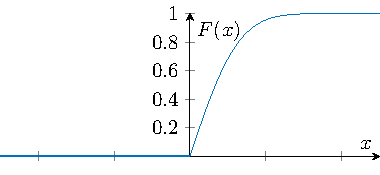
\includegraphics{./stoch_abbildungen/exponentialverteilung_verteilungsfunktion.pdf}
    \captionof{figure}{Verteilungsfunktion der Exponentialverteilung}
\end{center}

\begin{beispiel}
    Das Würfeln mit einem fairen, sechseitigen Würfel kann mittels einer reellen Zufallsvariablen
    \begin{equation*}
        \abb{X}{\menge{1,2,\dots, 6}}{\R} \mit x \mapsto x
    \end{equation*}
    modelliert werden. Es folgt als Verteilungsfunktion
    \begin{equation*}
    \begin{aligned}
    F(x) &= \P'(X \leq x) = \P(X^{-1}(-\infty,x]) = \P((-\infty,x]) \\
         &= \frac{1}{6}\sum_{i=1}^{6} \one_{\menge{i \leq x}}
    \end{aligned}
    \end{equation*}
\end{beispiel}

\begin{center}
    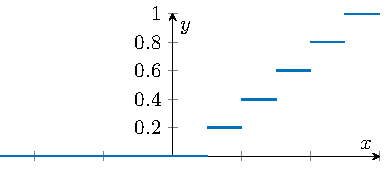
\includegraphics{./stoch_abbildungen/wuerfel_verteilungsfunktion.pdf}
    \captionof{figure}{Verteilungsfunktion des Würfelexperiments}
\end{center}

Diese Erkenntnisse lassen sich auch verallgemeinern:

\begin{satz}
    Ist $\P$ ein \WMass auf $(\R, \borel\R)$ und $F$ die zugehörige Verteilungsfunktion, so gelten
    \begin{enumerate}[nolistsep, topsep=-\parskip]
        \item $F$ ist monoton wachsend
        \item $F$ ist rechtsseitig stetig
        \item $\lim_{x\to -\infty} F(x) = 0$ und $\lim_{x\to \infty} F(x) = 1$
    \end{enumerate}
    Umgekehrt existiert zu jeder Funktion $\abb{F}{\R}{[0,1]}$ mit Eigenschaften (1) bis (3) eine reelle Zufallsvariable auf $((0,1), \borel((0,1)), \Uni((0,1))$ mit Verteilungsfunktion $F$.
\end{satz}

\begin{proof}
    Ist $F$ Verteilungsfunktion, so folgt mit \ref{satz: 1.4_rechenregeln}
    \begin{equation*}
        x \leq y \follows F(x) = \P((-\infty,x]) \overset{\ref{satz: 1.4_rechenregeln}.3}{\leq} \P((-\infty,y]) = F(y)
    \end{equation*}
    und
    \begin{equation*}
        \lim_{m \searrow c} F(x) = \lim_{m \searrow c} \P((-\infty, x]) \overset{\sigma\text{-Stetigkeit}}{=} \P((-\infty, c]) = F(c)
    \end{equation*}
    sowie
    \begin{equation*}
    \begin{aligned}
        \lim_{x\to -\infty} F(x) \overset{\ref{satz: 1.4_rechenregeln}.5}&{=} \P(\emptyset) \overset{\ref{satz: 1.4_rechenregeln}.1}{=} 0 \\
        \lim_{x\to \infty} F(x) \overset{\ref{satz: 1.4_rechenregeln}.5}&{=} \P(\R) = 1
    \end{aligned}
    \end{equation*}
    Umgekehrt wähle
    \begin{equation*}
        X(u) \defeq \inf \menge{x \in \R \colon F(x) \geq u}, \quad u \in (0,1)\\
    \end{equation*}
    Dann ist $X$ eine ``linkseitige Inverse'' von $F$ (auch \begriff{Quantilfunktion} oder \begriff{verallgemeinerte Inverse}).
    Wegen (3) gilt $-\infty < X(u) < \infty$ und zudem
    \begin{equation*}
        \menge{X \leq x} = (0, F(x)) \cap (0,1) \in \borel((0,1))
    \end{equation*}
    Da diese halboffene Mengen ein Erzeugendensystem von $\borel\R$ bilden, folgt bereits die Messbarkeit von $X$, also ist $X$ eine \ZV. Insbesondere hat die Menge $\menge{X \le x}$ gerade \person{Lebesgue}-Maß $F(x)$ und damit hat $X$ die Verteilungsfunktion $F$.
\end{proof}

\begin{korollar}
    Ist $\P$ \WMass auf $(\R, \borel\R)$ und $F$ die zugehörige Verteilungsfunktion. Dann besitzt $\P$ genau eine Dichtefunktion $\rho$, wenn $F$ stetig differenzierbar ist, denn dann gilt
    \begin{equation*}
        F(x) = \int_{0}^{x} \rho(x) \dx \quad \text{ bzw } \quad \rho(x) = F'(x)
    \end{equation*}
\end{korollar}

\begin{proof}
    Folgt aus \cref{satz: 1.8_mass_mit_dichte}, der \cref{def: 1.16_verteilungsfunktion} der Verteilungsfunktion und dem Eindeutigkeitssatz \labelcref{satz: 1.9_eindeutigkeitssatz}.
\end{proof}

\chapter{Erste Standardmodelle}
\begin{center}
    {\Large{\osfamily \itshape --- Diskrete Verteilungen ---}}
\end{center}
\section{Diskrete Gleichverteilungen}

\begin{*erinnerung}[\cref{def: 1.10_gleichverteilung}]
	Ist $\Omega$ endlich, so heißt \WMass mit Zähldichte $rho(\omega) = \frac{1}{\omega}$ für $\omega \in \Omega$ \begriff{(diskrete) Gleichverteilung} auf $\Omega \leadsto \Uni(\Omega)$
\end{*erinnerung}

Es gilt das für jedes $A \in \pows(\Omega)$
\begin{equation*}
	\P(A) = \frac{\# A}{\# \Omega}
\end{equation*}

Anwendungsbeispiele sind faires Würfeln, fairer Münzwurf, Zahlenlotto, ...
\section{Urnenmodelle}

Ein ``Urnenmodell'' ist eine abstrakte Darstellung von Zufallsexperimenten, bei denen zufällig Stichproben aus einer gegebenen Menge ``gezogen'' werden.
Eine Urne ist ein Behältnis in welchem sich farbige/nummerierte Kugeln befinden, die ansonsten ununterscheidbar sind.
Aus der Urne ziehe man blind/zufällig eine oder mehrere Kugeln und notiere ihre Farbe/Zahl.

\begin{center}
    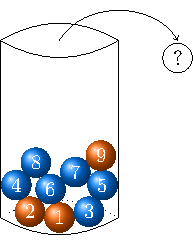
\includegraphics{./stoch_abbildungen/urne_mit_kugeln.pdf}
    \captionof{figure}{Urnenmodell mit nummerierten, farbigen Kugeln}
\end{center}

\subsection{Urnenmodell mit Zurücklegen: Multinomial-Verteilung}

Gegeben sei eine Urne mit $N$ Kugeln, verschiedenfarbig mit Farben aus $E$, wobei $\abs{E} \ge 2$ 

Man ziehe $n$ Stichproben/Kugeln, wobei nach jedem Zug die Kugel wieder zurückgelegt wird. Uns interessiert die Farbe in jedem Zug, setze also
\begin{equation*}
	\Omega = E^n \und \ereignisF = \pows\Omega 
\end{equation*}
Zur Bestimmung eines geeigneten Wahrscheinlichkeitsmaßes nummerieren wir die Kugeln mit $1,\dots, N$, so dass alle Kugeln der Farbe $a \in E$ eine Nummer aus $F_{a} \subset \menge{1,\dots, N}$ tragen. Würden wir die Nummern notieren, so wäre
\begin{equation*}
	\quer{\Omega} = \menge{1,\dots, N}^n \und \quer{\ereignisF} = \pows{\quer{\Omega}}
\end{equation*}
und wir könnten die Gleichverteilung $\quer{\P} = U(\quer{\Omega})$ als WMaß für einem einzelnen Zug verwenden. Für den Übergang zu $\Omega$ konstruieren wir  Zufallsvariablen. Die Farbe im $i$-ten Zug wird beschrieben durch
\begin{equation*}
	\bigabb{X_i}{\quer{\Omega}}{E}{\quer{\omega} = \left( \quer{\omega}_1, \dots, \quer{\omega}_n \right)}{a \enskip \text{ falls } \quer{\omega}_i \in F_a}
\end{equation*}
Der Zufallsvektor
\begin{equation*}
	\abb{X = (X_1, \dots, X_n)}{\quer{\Omega}}{\Omega}
\end{equation*}
beschreibt dann die Abfolge der Farben. Für jedes $\omega \in \Omega$ gilt dann
\begin{equation*}
	\menge{X = \omega} = F_{\omega_1} \times \cdots \times F_{\omega_n} = \bigtimes_{i=1}^{n} F_{\omega_i}
\end{equation*}
und damit
\begin{equation*}
    \P(\menge{\omega}) 
    = \quer{\P}(X^{-1}(\menge{\omega})) = \P(X=\omega)
    = \frac{\abs{F_{\omega_1}} \cdots \abs{F_{\omega_n}}}{\abs{\quer{\Omega}}}
    = \prod_{i=1}^{n} \frac{\abs{F_{\omega_i}}}{N} 
    \defqe \prod_{i=1}^{n} \rho(\omega_i)
\end{equation*}
Zähldichten, die sich als Produkt von Zähldichten schreiben lassen, werden auch als \begriff{Produktdichten} bezeichnet ($\nearrow$  \S 3 Unabhängigkeit).

Sehr oft interessiert uns bei einem Urnenexperiment nicht die Reihenfolge der gezogenen Farben, sondern nur die Anzahl der Kugeln in Farbe $a \in E$ nach $n$ Zügen. Dies entspricht
\begin{equation*}
	 \dach{\Omega} 
	 = \menge{k = (k_a)_{a \in E} \in \N_{0}^{\abs{E}} \colon \sum_{a \in E} k_a = n}
	 \und \dach{\ereignisF} = \pows{\dach{\Omega}}
\end{equation*}
Den Übergang $\Omega \to \dach{\Omega}$ beschreiben wir durch die Zufallsvariablen
\begin{equation*}
	\bigabb{Y_a(\omega)}{\Omega}{\N_{0}}%
    {\omega = (\omega_1,\dots, \omega_n)}%
    {\sum_{a \in E} \one_{\menge{a}}(\omega_i)} 
\end{equation*}
und
\begin{equation*}
	\abb{Y = (Y_a)_{a \in E}}{\Omega}{\dach{\Omega}}
\end{equation*}
Wir erhalten
\begin{equation*}
	\begin{aligned}
		\P(Y=k) &= \P(Y_a = k_a : a \in E) \\
		&= \sum_{\omega \in \Omega \colon Y(\omega) = k} \prod_{i=1}^ \rho(\omega_i)
		= \sum_{\omega \in \Omega \colon Y(\omega) = k} \prod_{a \in E} \rho(a)^{k_a} 
		= \binom{n}{\folge{k_a}[a \in E]} \prod_{a \in E} \rho(a)^{k_a}
	\end{aligned}
\end{equation*}
wobei
\begin{equation*}
	\binom{n}{(k_1 , \dots , k_l)} \defeq \begin{cases}
	\frac{n!}{k_1 ! \cdots k_l !} & \text{falls } \sum_{i=1}^l k_i = 1 \\
	0 & \text{sonst}
	\end{cases}
\end{equation*}
der Multinomialkoeffizient ist, welcher die Anzahl der Möglichkeiten beschreibt $n$ Objekte in $l$ Gruppen aufzuteilen, sodass die Gruppe $i$ gerade $k_i$ Objekte enthält.

\begin{definition}
	Sei $l \geq 2$, $p=(p_1 , \dots , p_l)$ eine Zähldichte und $n \in \N$, dann heißt die Verteilung auf 
	\begin{equation*}
		\menge{k=\folge{k_i}[i=1, \dots , l] \in \N_0^l : \sum_{i=1}^l k_i = 1}
	\end{equation*}
	mit Zähldichte
	\begin{equation*}
		m((k_1 , \dots , k_l)) = \binom{n}{k_1 , \dots , k_l} \prod_{i=1}^l p_i^{k_i}
	\end{equation*}
	\begriff{Mulitnomialverteilung} mit Parametern $n$ und $p$. Wir schreiben auch $\Multi(n,p)$.
\end{definition}

\begin{beispiel}
	Eine Urne enthalte nur schwarze (``1'') und weiße (``0'') Kugeln ($E = \menge{0,1}$) und es sei $\rho(1) = p$ gerade die Proportion der schwarzen Kugeln (Wahrscheinlichkeit bei einem Zug schwarz zu ziehen). Dann ist die Wahrscheinlichkeit in $n$ Zügen $k$-mal schwarz zu ziehen
	\begin{equation*}
		\binom{n}{k} \prod_{i=0,1} \rho(i)^{k_i} = \binom{n}{k} *p^k * (1-p)^{n-k}
	\end{equation*}
	Ein solches (wiederholtes) Experiment mit nur zwei möglichen Ergebnissen und feste Wahrscheinlichkeit $p \in [0,1]$ nennen wir auch (wiederholtes) \person{Bernoulli}-Experiment.
\end{beispiel}

\begin{definition}
	Sei $p \in [0,1]$ und $n \in \N$, dann heißt die Verteilung mit Zähldichte
	\begin{equation*}
		\rho(k) = \binom{n}{k} p^k (1-p)^{n-k} \qquad k \in \menge{0, 1 , \dots , n}
	\end{equation*}
	\begriff{Binomialverteilung} auf $\menge{0, \dots, n}$ mit Parameter $p$ (Erfolgswahrscheinlichkeit). Wir schreiben auch $\Bin(n,p)$. Im Fall $n=1$ nennen wir die Verteilung mit Zähldichte
	\begin{equation*}
		\rho(0) = 1-p \quad \rho(1) = p
	\end{equation*}
	auch \begriff{Bernoulliverteilung} mit Parameter $p$ und schreiben $\Bernoulli(p)$.
\end{definition}

\subsection{Urnenmodell ohne Zurücklegen: Hypergeometrische Verteilung}
Gegeben sei ein Urne mit $N$ Kugeln verschiedener Farben aus $E$ mit $\card{E} \geq 2$. Es werden $n \leq N$ Stichproben entnommen, wobei die gezogenen Kugeln nicht in die Urne zurückgelegt werden.

\begin{beispiel}
	Eine Urne enthalte $S$ schwarze (``1'') und $W$ weiße (``0'') Kugeln, d.h. $E = \menge{0,1}$ und $S+W=N$. Dann ist die Wahrscheinlichkeit in $n$ Zügen ohne Zurücklegen gerade $s$ schwarze und $w$ weiße Kugeln zu ziehen
	\begin{equation*}
		\rho(s) = \frac{\binom{W}{w} * \binom{S}{s}}{\binom{N}{n}} \qquad 0 \leq s \leq S, 0 \leq w \leq W, s+w=n, S+W=N
	\end{equation*}
\end{beispiel}

\begin{definition}
	Seien $N \in \N, W \leq N, n \leq N$. Dann heißt die Verteilung auf $\menge{0, \dots , n}$ mit Zähldichte 
	\begin{equation*}
		\rho(w) = \frac{\binom{W}{w} * \binom{N-W}{n-w}}{\binom{N}{n}} \qquad w = \max\menge{0 , n-N+W} , \dots \min\menge{W,n}
	\end{equation*}
	\begriff{Hypergeometrische Verteilung} mit Parametern $N,W$ und $n$. Wir schreiben auch $\Hyper(N,W,n)$.
\end{definition}
\section{Poisson-Approximation und -Verteilung}

$\Bin(n,p)$ ist zwar explizit und elementar definiert, jedoch für große $n$ mühsam auszuwerten. Für seltene Ereignisse ($n$ groß, $p$ klein) kann man daher eher den folgenden Satz anwenden.

\begin{satz}[Poisson-Approximation]
	Sei $\lambda > 0$ und $\folge{p_n}$ eine Folge in $[0,1]$ mit
	\begin{equation*}
		n*p_n \to \lambda,\quad n \to \infty
	\end{equation*}
	Dann gilt für alle $k \in \N_0$ für die Zähldichte der $\Bin(n,p_n)$-Verteilung
	\begin{equation*}
		\lim_{n \to \infty} \binom{n}{k} p_n^k (1-p_n)^{n-k} = e^{-\lambda} \frac{\lambda^k}{k!}
	\end{equation*}
\end{satz}
\begin{proof}
	Sei $k \in \N_{0}$ fix, dann
	\begin{equation*}
		\binom{n}{k} = \frac{n!}{k!(n-k)!} 
		= \frac{n^k}{k!}\frac{n(n-1)\cdots(n-k+1)}{n^k}
		= \frac{n^k}{k!}\cdot 1 \cdot (1-\frac{1}{n}\cdots \frac{k-1}{n})
		\overset{n \to \infty}{\widesim} \frac{n^k}{k!}
	\end{equation*}
	wobei $a(l) \overset{n \to \infty}{\sim} b(l) \Leftrightarrow \frac{a(l)}{b(l)} \xrightarrow{n\to \infty} 1$. Damit gilt
	\begin{equation*}
	\begin{aligned}
		\binom{n}{k}p^k (1-p)^{n-k} \overset{n \to \infty}&{\widesim} \frac{n^k}{k!}p_n^k(1-p_n)^{n-k}\\
		\overset{n \to \infty}&{\widesim} \frac{\lambda^k}{k!}(1-p_n)^n
		= \frac{\lambda^n}{k!}\brackets{1 - \frac{n*p_n}{n}}^n\\
		\overset{n \to \infty}&{\longrightarrow} \frac{\lambda^n}{k!}e^{-\lambda}
	\end{aligned}
	\end{equation*}
\end{proof}

Der erhaltene Grenzwert liefert die Zähldichte auf $\N_{0}$, denn 
\begin{equation*}
	\sum_{k=0}^{\infty}\frac{\lambda^k}{k!}e^{-\lambda} = e^{-\lambda}\sum_{k=0}^{\infty}\frac{\lambda^{k}}{k!} = e^{-\lambda}e^{\lambda} = 1
\end{equation*}

\begin{definition}
	Sei $\lambda >0$. Dann heißt das auf $(\N_{0}, \P(\N_{0}))$ definierte Wahrscheinlichkeitsmaß mit
	\begin{equation*}
		\P(\set{k}) = \frac{\lambda^k}{k!}e^{-\lambda} \quad k \in \N_{0},\notag
	\end{equation*}
	\begriff{Poissonverteilung} mit Parameter $\lambda$. Wir schreiben auch $\Poisson(\lambda)$.
\end{definition}

Die Poisson-Verteilung ist ein natürliches Modell für die Anzahl von zufälligen, seltenen Ereignissen (z.B. Tore im Fußballspiel, Schadensfälle einer Versicherung)


\chapter{Bedingte Wahrscheinlichkeiten und Unabhängigkeit}
\section{Bedingte Wahrscheinlichkeiten}
\begin{beispiel}\label{beispiel: 3_1_1_wuerfel}
	Das Würfeln mit zwei fairen, sechsseitigen Würfeln können wir mit 
	\begin{equation*}
		\Omega = \menge{(i,j) \colon i,j \in \menge{1,\dots,6}} \quad \und \quad \P = \Uni(\Omega)
	\end{equation*}
	modellieren. Da $\abs{\Omega} = 36$ gilt also $\P(\menge{\omega}) = \lfrac{1}{36}$ für alle $\omega \in \Omega$. Betrachten wir das Ereignis
	\begin{equation*}
		A = \menge{(i,j) \in \Omega \colon i + j = 8}
	\end{equation*}
	dann folgt $\P(A) = \frac{5}{36}$.	Werden die beiden Würfe nacheinander ausgeführt, so kann nach dem ersten Wurf eine Neubewertung der Wahrscheinlichkeit von $A$ erfolgen. Ist beispielsweise
	\begin{equation*}
		B = \menge{(i,j) \in \Omega, i = 4}
	\end{equation*} 
	eingetreten, so kann die Summe $8$ nur durch eine weitere $4$ realisiert werden, also mit Wahrscheinlichkeit
	\begin{equation*}
		\frac{1}{6} = \frac{\abs{A \cap B}}{\abs{B}}. 
	\end{equation*}
	Das Eintreten von $B$ führt also dazu, dass das Wahrscheinlichkeitsmaß $\P$ durch ein neues Wahrscheinlichkeitsmaß $\P_{B}$ ersetzt werden muss. Hierbei sollte gelten:
	\begin{align}
		&\text{Renormierung: } &&\P_{B} = 1 \label{eq: Renormierung} \tag{R}\\
		&\text{Proportionalität: } &&\text{Für alle } A \subseteq \F \mit A \subseteq B \text{ gilt } \P_{B}(A) = c_B * \P(A) \notag \\ 
		&&&\text{mit einer Konstante } c_B \label{eq: Proportionalitaet} \tag{P}
	\end{align}
\end{beispiel}

\begin{lemma}
	Sei $(\Omega, \F, \P)$ Wahrscheinlichkeitsraum und $B \in \F$ mit $\P(B) > 0$. Dann gibt es genau ein Wahrscheinlichkeitsmaß $\P_B$ auf $(\Omega, \F)$ mit den Eigenschaften \labelcref{eq: Renormierung} und \labelcref{eq: Proportionalitaet}. Dieses ist gegeben durch
	\begin{equation*}
		\P_B(A) = \frac{\P(A \cap B)}{\P(B)} \qquad \text{für alle } A \in \F
	\end{equation*}
\end{lemma}

\begin{proof}
	Offenbar erfüllt $\P_{B}$ wie definiert \labelcref{eq: Renormierung} und \labelcref{eq: Proportionalitaet}. Umgekehrt erfülle $\P_{B}$ die Eigenschaften \labelcref{eq: Renormierung} und \labelcref{eq: Proportionalitaet}. Dann folgt für $A \in \F$
	\begin{equation*}
		\P_B(A) = \P_{B}(A \cap B) + \underbrace{\P_{B}(A \setminus B)}_{= 0, \text{ wegen } \labelcref{eq: Renormierung}} \overset{\labelcref{eq: Proportionalitaet}}{=} c_B * \P(A \cap B).
	\end{equation*}
	Für $A=B$ folgt zudem aus \labelcref{eq: Renormierung}
	\begin{equation*}
		1 = \P_{B}(B) = c_B * \P(B)
	\end{equation*}
	also $c_B = \P(B)^{-1}$.
\end{proof}

%% % % % % % % % % % % % % % % % % % % % % % % % % % % 5th lecture % % % % % % % % % % % % % % % % % % % % % % % % % % %
%
\begin{definition} \label{def: 3_1_3_bedingteWahrscheinlichkeit}
	Sei $(\Omega, \F, \P)$ Wahrscheinlichkeitsraum und $B \in \F$ mit $\P(B) > 0$. Dann heißt
	\begin{equation*}
		\P(A \mid B) \defeq \frac{\P(A \cap B)}{\P(B)} \mit A \in \F
	\end{equation*}
	die \begriff{bedingte Wahrscheinlichkeit} von $A$ gegeben $B$.
	Falls $\P(B) = 0$, setze $\P(A \mid B) = 0$ für alle $A \in \F$.
\end{definition}

\begin{beispiel} %TODO ref
	In der Situation \cref{beispiel: 3_1_1_wuerfel} gilt $A \cap B = \menge{(4,4)}$ und damit
	\begin{equation*}
		\P(A \mid B) = \frac{\P(A \cap B)}{\P(B)} = \frac{\frac{1}{36}}{\frac{1}{6}} = \frac{1}{6}
	\end{equation*}
\end{beispiel}

Aus \cref{def: 3_1_3_bedingteWahrscheinlichkeit} ergibt sich das folgende Lemma.

\begin{lemma}[Multiplikationsformel] \label{lemma: 3_1_4_multiplikationsformel}
	Sei $(\Omega, \F, \P)$ ein Wahrscheinlichkeitsraum und $A_1, \dots, A_n \in \F$. Dann gilt
	\begin{equation*}
	\P(A_1 \cap \dots \cap A_n) = \P(A_1) \P(A_2 \mid A_1) \dots \P(A_n \mid A_1 \cap \dots \cap A_{n-1})
	\end{equation*}
\end{lemma}
\begin{proof}
	Ist $\P(A_1 \cap \dots \cap A_n) = 0$, so gilt auch $\P(A_n \mid A_1 \cap \dots \cap A_{n-1}) = 0$. Andernfalls sind alle Faktoren der rechten Seite ungleich Null und
	\begin{equation*}
	\begin{aligned}
		&\P(A_1) \P(A_2 \mid A_1) \dots \P(A_n \mid A_1 \cap \dots \cap A_{n-1}) \\
		= \enskip &\P(A_1) * \frac{\P(A_1 \cap A_2)}{\P(A_1)} \cdots \frac{\P(A_1 \cap \dots \cap A_n)}{\P(A_1 \cap \dots \cap A_{n-1}} \\
		= \enskip &\P(A_1 \cap \dots \cap A_n)
	\end{aligned}	
	\end{equation*}
\end{proof}

Stehen die $A_i$ in \cref{lemma: 3_1_4_multiplikationsformel} in einer (zeitlichen) Abfolge, so liefert Formel einen Hinweis wie Wahrscheinlichkeitsmaße für \begriff{Stufenexperimente} konstruiert werden können. Ein Stufenexperiment aus $n$ nacheinander ausgeführten Teilexperimenten lässt sich als \begriff{Baumdiagramm} darstellen.

\begin{center}
	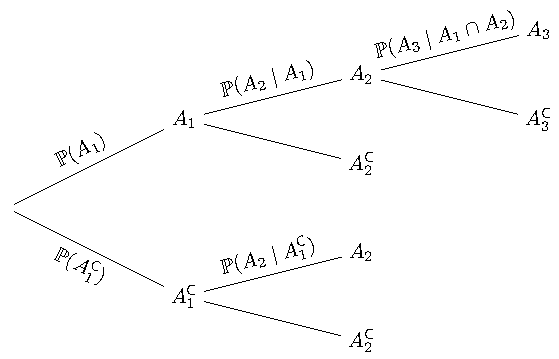
\includegraphics{./stoch_abbildungen/baum_1.pdf}
	\captionof{figure}{Darstellung eines Stufenexperiments}
\end{center}

\begin{satz}[ Wahrscheinlichkeitsmaß eines Stufenexperiments] \label{satz: 3_1_6_stufenexperiment}
	Gegeben seinen $n$ Ergebnisräume $\Omega_i = \menge{\omega_i (1), \dots, \omega_i (k)}, k \in \N \cup \menge{\infty}$ und es sei $\Omega = \Omega_1 \times \cdots \Omega_n$ der zugehörige Produktraum. Weiter seinen $\F_i$ $\sigma$-Algebren auf $\Omega_i$ und $\F = \bigotimes_{i=1}^n \F_i$ die Produkt-$\sigma$-Algebra auf $\Omega$. Setze $\omega = (\omega_1,\dots,\omega_n)$ und
	\begin{equation*}
	[\omega_1,\dots,\omega_m] \defeq \menge{\omega_1}\times \dots \times \menge{\omega_m} \times \Omega_{m+1} \times \cdots \times \Omega_{n} \qquad (m \leq n) 
	\end{equation*}
	und
	\begin{equation*}
		\P(\menge{\omega_m} \mid [\omega_1,\dots,\omega_{m-1}])
	\end{equation*}
	für die Wahrscheinlichkeit in der $m$-ten Stufe des Experiments $\omega_m$ zu beobachten, falls in den vorausgehenden Stufen $\omega_1,\dots,\omega_{m-1}$ beobachten wurden. Dann definiert
	\begin{equation*}
		\P(\menge{\omega}) \defeq \P(\menge{\omega_1}) \prod_{m=2}^{n}\P\brackets{\menge{\omega_m} \mid [\omega_1, \dots, \omega_{m-1}]}
	\end{equation*}
	ein Wahrscheinlichkeitsmaß auf $(\Omega, \F, \P)$.
\end{satz}
\begin{proof}
	Nachrechnen!
\end{proof}

\begin{beispiel}[\person{Polya}-Urne]
	Gegeben sei eine Urne mit $s$ schwarzen und $w$ weißen Kugeln. Bei jedem Zug wird die  gezogene Kugel zusammen mit $c \in \N_0 \cup \menge{-1}$ weiteren Kugeln derselben Farbe zurückgelegt.
	\begin{itemize}
		\item $c=0$: Urnenmodell mit Zurücklegen
		\item $c=-1$: Urnenmodell ohne Zurücklegen
	\end{itemize}
	Beide haben wir schon in Kapitel 2.2 gesehen. 
	Sei deshalb $c\in \N$ (Bsp. Modell für zwei konkurrierende Populationen). Ziehen wir $n$-mal, so haben wir ein $n$-Stufenexperiment mit 
	\begin{equation*}
		\Omega = \menge{0,1}^n \mit \text{ 0 = ``weiß'', 1 = ``schwarz''} \quad (\Omega_i = \menge{0,1})
	\end{equation*}
	Zudem gelten im ersten Schritt
	\begin{equation*}
		\P(\menge{0}) = \frac{w}{s+w} \und \P(\menge{1}) = \frac{s}{s+w}
	\end{equation*}
	sowie
	\begin{equation*}
		\P(\menge{\omega_m} \mid [\omega_1, \dots \omega_{m-1}]) = 
		\begin{cases}
		\frac{w+c \brackets{m-1 - \sum_{i=1}^{m-1}\omega_i}}{s+w+c(m-1)} & \omega_m = 0\\
		\frac{s + c\sum_{i=1}^{m-1}\omega_i}{s+w+c(m-1)} & \omega_m = 1
		\end{cases}
	\end{equation*}
	Mit \cref{satz: 3_1_6_stufenexperiment} folgt als Wahrscheinlichkeitsmaß auf $(\Omega, \pows(\Omega))$
	\begin{equation*}
	\begin{aligned}
		\P(\menge{(\omega_1, \dots, \omega_n)}) 
		&= \P(\menge{\omega_1}) \prod_{m=2}^n \P(\menge{\omega_m}\mid [\omega_1,\dots,\omega_{m-1}]) \\
		&= \frac{\prod_{i=0}^{l-1}(s+c * i) \, \prod_{j=0}^{n-l-1}(w + c * j)}{\prod_{i=0}^n (s+w+c * i)}
	\end{aligned}
	\end{equation*}
	mit $l=\sum_{i=1}^n \omega_i$. Definiere wir nun die Zufallsvariable
	\begin{equation*}
		\abb{S_n}{\Omega}{\N_0} \mit (\omega_1, \dots, \omega_n) \mapsto \sum_{i=1}^n \omega_i
	\end{equation*}
	welche die Anzahl der gezogenen schwarzen Kugeln modelliert, so folgt
	\begin{equation*}
		\P(S_n = l) = \binom{n}{l} \frac{\prod_{i=0}^{l-1}(s+c * i) \, \prod_{j=0}^{n-l-1}(w + c * j)}{\prod_{i=0}^n(s+w+c * i)}
	\end{equation*}
	Mittels $a \defeq \lfrac{s}{c}$ und $b \defeq \lfrac{w}{c}$ folgt
	\begin{equation*}
		\begin{aligned}
			\P(S_n = l) = \binom{n}{l} \frac{\prod_{i=0}^{l-1}(-a-i)\prod_{j=0}^{n-l-1}(-b-j)}{\prod_{i=0}^n (-a-b-i)} = \frac{\binom{-a}{l}\binom{-b}{n \cdot l}}{\binom{-a-b}{n}} \mit l \in \menge{0,\dots,n} 
		\end{aligned}
	\end{equation*}
	Dies ist die \begriff{\person{Polya}-Verteilung} auf $\menge{0,\dots,n}$ ($n \in \N$) mit Parametern $a,b > 0$.
\end{beispiel}

\begin{beispiel} \label{beispiel_3_1_8_multiplechoice}
	Ein Student beantwortet eine Multiple-Choice-Frage mit vier Antwortmöglichkeiten, eine davon ist richtig. Er kennt die richtige Antwort mit Wahrscheinlichkeit $\lfrac{2}{3}$. Wenn er die richtige Antwort kennt, so wählt er diese aus. Andernfalls wählt er zufällig (gleichverteilt) eine Antwort. Betrachten wir 
	\begin{equation*}
		W = \menge{\text{richtige Antwort gewusst}} \und 
		R = \menge{\text{Richtige Antwort gewählt}}
	\end{equation*}
	Dann gilt
	\begin{equation*}
		\P(W) = \frac{2}{3} \qquad \P(R \mid W) = 1 \qquad \P(R \mid W^\complement) = \frac{1}{4}
	\end{equation*}
	Angenommen der Student gibt die richtige Antwort. Mit welcher Wahrscheinlichkeit hat er diese gewusst? $\longrightarrow \enskip \P(W \mid R) = \text{ ?}$
\end{beispiel}

\begin{satz} \label{satz: 3_1_9_totaleW_bayes}
	Sei $(\Omega, \F, \P)$ ein Wahrscheinlichkeitsraum und $\Omega = \bigcup_{i \in I} B_i$ eine höchstens abzählbare Zerlegung in paarweise disjunkte Ereignisse $B_i \in \F$.
	\begin{enumerate}
		\item \textit{Satz von der totalen Wahrscheinlichkeit:} Für alle $A \in \F$ gilt
		\begin{align}
			\P(A) = \sum_{i\in I} \P(A\mid B_i) * \P(B_i) \label{eq: totaleWkeit}
		\end{align} 
		\item \textit{Satz von Bayes:} Für alle $A \in \F$ mit $\P(A) > 0$ und alle $k \in I$ gilt
		\begin{align}
			\P(B_k \mid A) = \frac{\P(A \mid B_k) * \P(B_k)}{\sum_{i\in I}\P(A\mid B_i) * \P(B_i)} \label{eq: bayes}
		\end{align}
	\end{enumerate}
\end{satz}

\begin{proof}
	Es gilt:
	\begin{equation*}
		\sum_{i\in I} \P(A\mid B_i) * \P(B_i) = \sum_{i\in I}\frac{\P(A \cap B_i)}{\P(B_i)} * \P(B_i) = \sum_{i\in I} \P(A \cap B_i) \overset{\sigma-Add.}{=} \P(A)
	\end{equation*}
	und
	\begin{equation*}
	\P(B_k \mid A) = \frac{\P(A \cap B_k)}{\P(A)} = \frac{\P(A \mid B_k) * \P(B_k)}{\P(A)}
	\end{equation*}
	also folgt (b) aus (a).
\end{proof}

\begin{beispiel}
	In der Situation von \cref{beispiel_3_1_8_multiplechoice} folgt mit \labelcref{eq: totaleWkeit}
	\begin{equation*}
	\begin{aligned}
		\P(R) 
		&= \P(R \mid W) * \P(W) + \P(R \mid W^\complement) * \P(W^\complement) \\
		&= 1 \cdot \frac{2}{3} + \frac{1}{4} * \frac{1}{3} = \frac{3}{4}
	\end{aligned}
	\end{equation*}
	und mit \labelcref{eq: bayes}
	\begin{equation*}
		\P(W \mid R) = \frac{\P(R \mid W) * \P(W)}{\P(R)} = \frac{1 * \frac{2}{3}}{\frac{3}{4}} = \frac{8}{9}
	\end{equation*}
	für die gesuchte Wahrscheinlichkeit.
	\begin{center}
		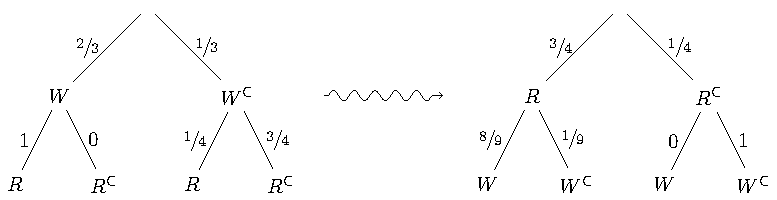
\includegraphics{./stoch_abbildungen/baum_2.pdf}
		\captionof{figure}{Bedingte Wahrscheinlichkeit im Baumdiagramm}
	\end{center}
\end{beispiel}
\section{Stochastische Unabhängigkeit} \label{sec: unabhaengigkeit}
In vielen Fällen besagt die Intuition über verschiedene Zufallsexperimente / Ereignisse, dass diese sich \textit{nicht} gegenseitig beeinflussen. Für solche $A,B \in \F$ mit $\P(A) > 0$ und $\P(B) > 0$ sollte gelten
\begin{equation*}
	\P(A\mid B) = \P(A) \quad \und \quad \P(B\mid A) = \P(B).
\end{equation*}

\begin{definition} \label{def: 3_2_11}
	Sei $(\Omega, \F, \P)$ Wahrscheinlichkeitsraum. Zwei Ereignisse $A,B \in \F$ heißt \begriff{(stochastisch) unabhängig} bezüglich $\P$, falls
	\begin{equation*}
		\P(A\cap B) = \P(A) * \P(B)
	\end{equation*}
	Wir schreiben auch $A \upmodels B$.
\end{definition}

\begin{beispiel}
	Wir betrachten wieder das Würfeln mit 2 fairen, sechsseitigen Würfeln. 
	\begin{equation*}
		\Omega = \menge{(i,j) \mid i,j \in\menge{1,\dots,n}} \qquad 
		\F = \pows\Omega \qquad 
		\P = \Uni(\Omega)
	\end{equation*}
	Betrachte
	\begin{equation*}
	\begin{aligned}
		A &\defeq \menge{(i,j) \in \Omega \colon i \text{ gerade}}\\
		B &\defeq \menge{(i,j) \in \Omega \colon j \leq 2}
	\end{aligned}
	\end{equation*}
	In diesem Fall, erwarten wir intuitiv die Unabhängigkeit von $A$ und $B$.
	In der Tat ist $\P(A) = \lfrac{1}{2}$, $\P(B) = \lfrac{1}{3}$ und $\P(A\cap B) = \lfrac{1}{6}$, womit $\P(A \cap B) = \P(A) * \P(B)$ erfüllt ist.
	Betrachte nun
	\begin{equation*}
	\begin{aligned}
		C &\defeq \menge{(i,j) \in \Omega \colon i + j = 7}\\
		D &\defeq \menge{(i,j) \in \Omega \colon i = 6}
	\end{aligned}
	\end{equation*}
	Dann gilt $\P(C) = \lfrac{1}{6}$ und $\P(D) = \lfrac{1}{6}$. Wegen $C \cap D = \menge{(6,1)}$ folgt
	\begin{equation*}
		\P(C\cap D) = \frac{1}{36} = \frac{1}{6} * \frac{1}{6} = \P(C) * \P(D)
	\end{equation*}
	$C$ und $D$ sind also \textit{stochastisch} unabhängig, obwohl eine kausale Abhängigkeit vorliegt.
\end{beispiel}

\begin{definition}
	Sei $(\Omega, \F, \P)$ ein Wahrscheinlichkeitsraum und $I \neq \emptyset$ eine endliche Indexmenge. Dann heißt die Familie $(A_i)_{i \in I}$ von Ereignissen in $\F$ \begriff{unabhängig} bezüglich $\P$, falls für alle $\emptyset \neq J \subseteq I$ gilt
	\begin{equation*}
		\P\brackets{\bigcap_{i \in J} A_i} = \prod_{i \in J} \P(A_i)
	\end{equation*}
	Offensichtlich impliziert die Unabhängigkeit einer Familie die paarweise Unabhängigkeit je zweier Familienmitglieder nach \cref{def: 3_2_11}. Umgekehrt gilt dies nicht.
\end{definition}

\begin{beispiel}[Abhängigkeit trotz paarweiser Unabhängigkeit]
	Wir betrachten ein zweifaches Bernoulliexperiment mit Erfolgswahrscheinlichkeit $\lfrac{1}{2}$, d.h.
	\begin{equation*}
		\Omega = \menge{0,1}^2 \qquad \F = \pows\Omega \qquad \P = \Uni(\Omega)
	\end{equation*}
	sowie
	\begin{equation*}
	\begin{aligned}
		A &= \menge{1} \times \menge{0,1} \qquad &&\text{(Münzwurf: erster Wurf ist Zahl)}\\
		B &= \menge{0,1} \times \menge{1} &&\text{(Münzwurf: zweiter Wurf ist Zahl)}\\
		C &= \menge{(0,0), (1,1)} &&\text{(beide Würfe haben selbes Ergebnis)}
	\end{aligned}
	\end{equation*}
	Dann gelten $\P(A) = \lfrac{1}{2} = \P(B) = \P(C)$ und
	\begin{equation*}
	\begin{aligned}
		\P(A\cap B) &= \P(\menge{(1,1)}) = \lfrac{1}{4} = \P(A) * \P(B)\\
		\P(A\cap C) &= \P(\menge{(1,1)}) = \lfrac{1}{4} = \P(A) * \P(C)\\
		\P(B\cap C) &= \P(\menge{(1,1)}) = \lfrac{1}{4} = \P(B) * \P(C)
	\end{aligned}
	\end{equation*}
	Daraus folgt also paarweise Unabhängigkeit. Jedoch ist
	\begin{equation*}
		\P(A \cap B \cap C) = \P(\menge{(1,1)}) = \frac{1}{4} \neq \P(A) * \P(B) * \P(C)
	\end{equation*}
	und $A,B,C$ sind \textit{nicht} stochastisch unabhängig.
\end{beispiel}

\begin{definition}[Unabhängige $\sigma$-Algebren] \label{3_15_def}
	Seien $(\Omega, \F,\P)$ ein Wahrscheinlichkeitsraum, $I \neq \emptyset$ eine Indexmenge und $(E_i, \Ecal_i)$ Messräume.
	\begin{enumerate}[leftmargin=*]
		\item Die Familie $\F_i \subset \F (i \in I)$, heißen \begriff{unabhängig}, wenn für die $\emptyset \neq J \subseteq I$ mit $\abs{J} < \infty$ gilt
		\begin{equation*}
			\P\brackets{\bigcap_{i \in J} A_i} = \prod_{i \in J} \P(A_i) \qquad \text{ für beliebige } A_i \in \F_i (i \in J)
		\end{equation*}
		\item Die Zufallsvariable $\abb{X_i}{(\Omega, \F)}{(E_i, \Ecal_i)} (i \in I)$, heißen \begriff{unabhängig}, wenn die $\sigma$-Algebren
		\begin{equation*}
			\sigma(X_i) = X^{-1}(\Ecal_i) = \menge{\menge{X_i \in F} \colon F \in \Ecal_i} \quad (i \in I)
		\end{equation*}
		unabhängig sind.
	\end{enumerate}
\end{definition}

\begin{lemma}[Zusammenhang der Definitionen]
	\label{3_16_lemma}
	Sei $(\Omega,\F,\P)$ ein Wahrscheinlichkeitsraum, $I \neq \emptyset$, $A_i \in \F_i$ für alle $i \in I$. 
	Die folgenden Aussagen sind äquivalent:
	\begin{enumerate}[nolistsep]
		\item Die Ereignisse $A_i$ ($i \in I$) sind unabhängig. 
		\item Die $\sigma$-Algebren $\sigma(A_i)$ ($i \in I$) sind unabhängig.
		\item Die Zufallsvariablen $\one_{A_i}$ ($i \in I$) sind unabhängig.
	\end{enumerate}
\end{lemma}
\begin{proof}
	Da die Unabhängigkeit über endliche Teilemengen definiert ist, können wir oBdA $I = \menge{1, \dots, n}$ annehmen. 
	\begin{itemize}[leftmargin=*, nolistsep]
		\item Da $\sigma(\one_{A_i}) = \sigma(A_i)$ folgt die Äquivalenz von (2) und (3) direkt aus \cref{3_15_def}.
		\item Zudem ist (2) $\to$ (1) klar.
		\item Für (1) $\to$ (2) genügt es zu zeigen, dass
		\begin{equation*}
			A_1, \dots, A_n \text{ unabhängig } \Rightarrow B_1, \dots, B_n \text{ unabhängig mit } B_i \in \menge{\emptyset, A_i, A_i^\complement, \Omega}
		\end{equation*}
		Rekursiv folgt dies bereits aus
		\begin{equation*}
			A_1,\dots, A_n \text{ unabhängig } \Rightarrow B_1, A_2, \dots, A_n \text{ unabhängig mit } B_1 \in \menge{\emptyset, A_1, A_1^\complement, \Omega}.
		\end{equation*}
		Für $B_1 \in \menge{\emptyset, A_1, \Omega}$ ist dies klar.\\
		Sei also $B_1 = A_1^\complement$ und $J \subseteq I$, $J \neq \emptyset$. Falls $1 \notin J$, ist nichts zu zeigen. Sei $1 \in J$, dann gilt mit $A = \bigcap_{i\in J, i \neq 1} A_i$ sicherlich
		\begin{equation*}
			\begin{aligned}
				\P\brackets{A_1^\complement \cap A} 
				&= \P(A \setminus (A_1 \cap A))\\
				&= \P(A) - \P(A_1 \cap A)\\
				&= \prod_{i\in J \setminus \menge{1}} \P(A_i) - \prod_{i\in J}(A_i) \\
				&= (1- \P(A_1))\prod_{i\in J\setminus \menge{1}} \P(A_i)\\
				&= \P\brackets{A_1^\complement} \prod_{i\in J \setminus \menge{1}} \P(A_i)
			\end{aligned}
		\end{equation*}
	\end{itemize}
\end{proof}

Insbesondere zeigt \cref{3_16_lemma}, dass wir in einer Familie unabhängiger Ereignisse beliebig viele Ereignisse durch ihr Komplement, $\emptyset$ oder $\Omega$ ersetzen können ohne die Unabhängigkeit zu verlieren.

\begin{satz}
	\label{3_17_satz}
	Sei $(\Omega, \F, \P)$ Wahrscheinlichkeitsraum und $\F_i \subseteq \F, i \in I$, seien $\cap$-stabile Familien von Ereignissen. Dann gilt
	\begin{equation*}
		\F_i (i \in I) \text{ unabhängig } \equivalent \sigma(\F_i) (i \in I) \text{ unabhängig}. 
	\end{equation*}
\end{satz}

\begin{proof}
	oBdA sei $I = \menge{1, \dots, n}$ und $\Omega \in \F_i, i \in I$.
	\begin{proof-equivalence}[leftmargin=*, nolistsep]
		\rueckrichtung trivial, da $\F_i \subseteq \sigma(\F_i)$ und das Weglassen von Mengen erlaubt ist.
		\hinrichtung zeigen wir rekursiv
		\begin{enumerate}[label=(\roman*), nolistsep]
			\item Wähle $F_i \in \F_i, i = 2, \dots,n$ und definiere für $F \in \sigma(\F_i)$ die endlichen Maße
			\begin{equation*}
				\mu(F) = \P\brackets{ F \cap F_2 \cap \cdots \cap F_n} \und \nu(F) = \P(F) \, \P(F_2) \, \dots \, \P(F_n)
			\end{equation*}
			\item Da die Familien $\F_i$ unabhängig sind, gilt
			$\mu\mid_{\F_1} = \nu\mid_{\F_1}$.
			Nach dem Eindeutigkeitssatz für Maße (\cref{satz: 1.9_eindeutigkeitssatz}) folgt $\mu\mid_{\sigma(\F_1)} = \nu\mid_{\sigma(\F_1)}$ also
			\begin{equation*}
				\P\brackets{ F \cap F_2 \cap \cdots \cap F_n} = \P(F) \P(F_2) \dots \P(F_n)
			\end{equation*}
			für alle $F \in \sigma(\F_i)$ und $F_i \in \F_i, i = 1, \dots, n$. Da $\Omega \in \F_i$ für alle $i$ gilt die erhaltene Produktformel auf für alle Teilemengen $J \subseteq I$.\\
			Also sind $\sigma(\F_1), \F_2, \dots, \F_n$ unabhängig.
			\item Wiederholtes Anwenden von (i) und (ii) liefert den Satz.
		\end{enumerate}
	\end{proof-equivalence}
\end{proof}
%
Mit \cref{3_17_satz} folgen:

\begin{korollar}	\label{3_18_kor}
	Sei $(\Omega,\F,\P)$ ein Wahrscheinlichkeitsraum und $\F_{i,j} \subseteq \F$ mit $1 \le i \le n, 1 \le j \le m(i)$ unabhängige, $\cap$-stabile Familien.
	Dann sind auch
	\begin{equation*}
		\G_i = \sigma(\F_{i,1}, \dots , \F_{i,m(i)}), \quad 1 \le i \le n
	\end{equation*}
	unabhängig.
\end{korollar}
\begin{proof}
	oBdA sei $\Omega \in \F_{i,j} \enskip \forall i,j$, da $\Omega$ die Unabhängigkeit nach \cref{3_16_lemma} nicht zerstört.
	Dann sind die Familien 
	\begin{equation*}
		\F_i^\cap \defeq \menge{F_{i,1} \cap \cdots \cap F_{i,m(i)} : F_{i,j} \in \F_{i,j}, 1 \le j \le m(i)} \enskip (1 \le i \le n)
	\end{equation*}
	$\cap$-stabil, unabhängig und es gilt $\F_{i,1}, \dots , \F_{i,m(i)} \subseteq \F_i^\cap$ (vgl. Hausaufgabe). Nach \cref{3_17_satz} sind auch $\sigma(\F_i^\cap)$ unabhängig. Damit folgt die Behauptung, da aus 
	\begin{equation*}
		\F_{i,1}, \dots , \F_{i,m(i)} \subseteq \F_i^\cap \subseteq \sigma(\F_{i,1}, \dots , \F_{i,m(i)}) = \G_i
	\end{equation*} unter Anwendung des Erzeugenden-Operators $\G_i = \sigma(\F_{i,1}, \dots , \F_{i,m(i)}) \subseteq \sigma(\F_i^\cap) \subseteq \G_i$ folgt, d.h. $\sigma(\F_i^\cap) = \G_i$.
\end{proof}

\begin{korollar} \label{3_19_korollar}
	Sei $(\Omega,\F,\P)$ ein Wahrscheinlichkeitsraum und $\abb{X_{i,j}}{\Omega}{E}$ ($1 \le i \le n, 1 \le j \le m(i)$)
	unabhängige Zufallsvariablen. Zudem seinen $\abb{f_i}{E^{m(i)}}{\R}$ messbar. Dann sind auch die Zufallsvariablen $f_i(X_{i,1}, \dots, X_{i,m(i)})$ mit $1 \le i \le n$ unabhängig.
\end{korollar}
\begin{proof}
	Setze $\F_{i,j} = \sigma(X_{i,j})$ und $\G_i = \sigma(\F_{i,1} , \dots , \F_{i,m(i)})$. Dann sind nach \cref{3_18_kor} die $\G_i$ ($i = 1, \dots , n)$ unabhängig. Zudem ist $Y_i \defeq f_i(X_{i,1}, \dots , X_{i,m(i)})$ $\G_i$-messbar, also $\sigma(Y_i) \subseteq \G_i$. Damit erben die $Y_i$ die Unabhängigkeit der $\G_i$.
\end{proof}

\begin{beispiel}
	Seien $X_1, \dots, X_n$ unabhängige, reelle Zufallsvariablen. Dann sind auch
	\begin{equation*}
	Y_1 = X_1, Y_2 = X_2 + \cdots + X_n
	\end{equation*}
	unabhängig.
\end{beispiel}

\begin{satz}[Unabhängigkeit von Zufallsvariablen]
	\label{3_21_satz}
	Seien $(\Omega, \F, \P)$ ein Wahrscheinlichkeitsraum und $\abb{X_1, \dots, X_n}{(\Omega,\F)}{(E, \Ecal)}$ Zufallsvariablen. Dann sind äquivalent:
	\begin{enumerate}[label=(\arabic*), nolistsep]
		\item $X_1 , \dots , X_n$ sind unabhängig.
		\item $\P(X_1 \in A_1 , \dots , X_n \in A_n) = \prod_{i=1}^n \P(X_i \in A_i) \quad \forall A_1, \dots , A_n \in \Ecal$
		\item Die gemeinsame Verteilung der $X_i$ entspricht dem Produktmaß der einzelnen Verteilungen
		\begin{equation*}
			\P_{X_1 , \dots , X_n} = \P_{X_1} \otimes \dots \otimes \P_{X_n}
		\end{equation*}
	\end{enumerate}
\end{satz}
\begin{proof}
	per Ringschluss 
	\begin{description}[nolistsep]
		\item [(1 $\boldsymbol{\Rightarrow}$ 2)] Seien $A_1, \dots, A_n \in \Ecal$ beliebig. Dann gilt per Definition
		\begin{equation*}
			\begin{aligned}
				\P_{X_1 , \dots , X_n}(A_1 \times \dots A_n) 
				&= \P(X_1 in A_1, \dots , X_n \in A_n) \\
				&= \P\brackets{\bigcap_{i=1}^n \menge{X_i \in A_i}} \\
				&= \prod_{i=1}^n \P(X_i \in A_i) \\
				&= \prod_{i=1}^n \P_{X_i}(A_i) \\
				&= \brackets{\bigotimes_{i=1}^n \P_{X_i}} \brackets{A_1 \times \dots \times A_n}
			\end{aligned}
		\end{equation*}
		\item [(2 $\boldsymbol{\Rightarrow}$ 3)] Aus der obigen Gleichung sehen wir, dass (2) bereits (3) impliziert für alle Rechtecke $A_1 \times \dots \times A_n$. Da die Familie der Rechtecke $\cap$-stabil ist und $\Ecal^{\otimes n}$ erzeugt, folgt die Aussage aus dem Eindeutigkeitssatz für Maße.
		\item [(3 $\boldsymbol{\Rightarrow}$ 1)] Es sei $J \subseteq \menge{1, \dots, n}$ und 
		\begin{equation*}
			A_i \defeq \begin{cases}
			\text{beliebig in } \Ecal & \text{falls } i \in J \\
			E & \text{falls } i \notin J
			\end{cases}
		\end{equation*}
		Dann ist
		\begin{equation*}
			\begin{aligned}
			\P(X_i \in A_i : i \in  J) 
			&= \P(X_i \in A_i : i = 1 , \dots , n) \\
			&= \prod_{i=1}^n \P(X_i \in A_i) \\
			&= \prod_{i \in J} \P(X_i \in A_i)
			\end{aligned}
		\end{equation*}
	\end{description}
\end{proof}

\begin{beispiel}
	Im Urnenmodell mit Zurücklegen hat der Vektor $X = (X_1, \dots , X_n)$ mit $X_i$ = Farbe im $i$-ten Zug als Zähldichte die Produktdichte der $X_i$. $X_1 , \dots , X_n$ sind also unabhängig.
\end{beispiel}


\end{document}